% !TEX encoding = UTF-8 Unicode
\chapter{Elastic rod : variational approch}

% #######################################################
\section{Introduction}
% #######################################################

In this section a novel element with 4 degrees of freedom accounting for torsion and bending behaviours is presented. The beam is considered in Kirchhoff's theory framework, so that it is supposed to be inextensible and its sections are supposed to remain orthogonal to the centreline during deformation. The reduction from the classic 6-DoF model to this 4-DoF model is achieved by an appropriate curve-angle representation based on a relevant curve framing. Energies are then formulated and leads to internal forces and moments acting on the beam. The static equilibrium is deduced from a damped fictitious dynamic with an adapted dynamic relaxation algorithm.

Basile \cite{Bergou2010}

Basile \cite{Bergou2008}
Je
Basile \cite{Audoly2000}

Sina \cite{Nabei2014}

\cite{Fuller1978}, \cite{deVries2005},  \cite{Vauquelin2000}, \cite{Berger2009}

Dynamic relaxation :
\cite{Lewis2003}
En particulier,voir pour un comparatif avec une méthode implicite.

\note{
\begin{enumerate}
\item quaternion pour piloter les input / ouput ?
\item calcul de la hessienne au moins pour les $\theta$ comme Audoly. Ne serait-ce pas possible pour les $x$ ?  Avec ma technique du transport parallèle il me semble pourvoir avoir accès au DL à  l'ordre 2 ...
\item Formulation pour les efforts ponctuels / moments extérieurs en vue d'une résolution par minimisation. Voir F. Bertails
\item prise en compte des contraintes => méméthide des multiplicateurs de lagrange
\end{enumerate}



}



% #######################################################
\section{Kirchhoff rod}
The geometric configuration of the rod is described by its centerline $\vect{x}(s)$ and its cross sections. The centerline is parameterized by its arc-length. Cross sections orientations are followed along the centerline by their material frame $\{\vect{d}_3 (s),\vect{d}_1 (s),\vect{d}_2 (s)\}$ which is an adapted orthonormal moving frame aligned to section's principal axes of inertia. Here, \guil{adapted} means $\vect{d}_3 (s)=\vect{x}'(s)=\vect{t}(s)$ is aligned to the centerline's tangent. In the literature, this description is also known as a \emph{Cosserat Curve} \cite{Spillmann2007}.

\subsection{Inextensibility}
Note the previous description is only valid for inextensible rods in order to follow material points by their arc-length indifferently in their rest or deformed configuration. As explained in \cite{Audoly2010}, this hypothesis is usually relevant for slender beams. Indeed, in practice, if a slender member faces substantial axial strain the bending behaviour would become negligible due to the important difference between axial and bending stiffness. The length of the rod will be denoted $L$ and the arc-length $s$ will vary (with no loss of generality) in $[0,L]$.

\subsection{Euler-Bernouilli}
Strains are supposed to remain small so that material frame remains orthogonal to the centerline in the deformed configuration. Thus, differentiating the conditions of orthonormality leads to the following differential equations governing the evolution of $\{\vect{d}_3 (s),\vect{d}_1 (s),\vect{d}_2 (s)\}$ along the centerline :
\begin{equation} \label{eq:3_1}
	\begin{bmatrix}
		\mathbf{d'_{3}}(s) \\
		\mathbf{d'_{1}}(s) \\
		\mathbf{d'_{2}}(s)
	\end{bmatrix}
	=
	\begin{bmatrix}
		0 & \kappa_{2}(s) & -\kappa_{1}(s) \\
		-\kappa_{2}(s) & 0 & \tau(s) \\
		\kappa_{1}(s) & -\tau(s) & 0
	\end{bmatrix}
	\begin{bmatrix}
		\mathbf{d_{3}}(s) \\
		\mathbf{d_{1}}(s) \\
		\mathbf{d_{2}}(s)
	\end{bmatrix}
\end{equation}

\note{La théorie des poutres est une application de la théorie de l'élasticité isotrope. Pour mener les calculs de résistance des matériaux, on considère les hypothèses suivantes :

(1) hypothèse de Bernoulli : au cours de la déformation, les sections droites restent perpendiculaires à  la courbe moyenne ;

(2) les sections droites restent planes selon Navier-Bernoulli (pas de gauchissement).

L'hypothèse de Bernoulli permet de négliger le cisaillement dans le cas de la flexion : le risque de rupture est alors due à  l'extension des fibres situées à  l'extérieur de la flexion, et la flèche est due au moment fléchissant. Cette hypothèse n'est pas valable pour les poutres courtes car ces dernières sont hors des limites de validité du modèle de poutre, à  savoir que la dimension des sections doit être petite devant la longueur de la courbe moyenne. Le cisaillement est pris en compte dans le modèle de Timoshenko et Mindlin.}

\subsection{Darboux vector}
Those equations can be formulated with the \emph{Darboux vector} of the chosen material frame, which represents the rotational velocity of the frame along $\vect{x}(s)$ :
\begin{gather}
	\vect{d}'_{i}(s) = \vect{\Omega}_m(s) \times \vect{d}_i(s)
	\quad,\quad
	\vect{\Omega}_m(s)
	=
	\begin{bmatrix}
		\tau(s) \\
		\kappa_{1}(s) \\
		\kappa_{2}(s)
	\end{bmatrix}
\end{gather}
Where $\kappa_1(s)$, $\kappa_2(s)$ and $\tau(s)$ represent respectively the rate of rotation of the material frame around the axis  $\vect{d}_1 (s)$, $\vect{d}_2 (s)$ and $\vect{d}_3 (s)$.

\subsection{Curvatures and twist}
The material curvatures are denoted $\kappa_1(s)$ and $\kappa_2(s)$ and represent the rod's flexion in the principal planes respectively normal to $\vect{d}_1(s)$ and $\vect{d}_2(s)$ .The material twist is denoted $\tau(s)$ and represents the section's rate of rotation around $\vect{d}_3(s)$. Those scalar functions measure directly the strain as defined in Kirchhoff's theory (Figure 4). Recall that the Frenet frame $\{\vect{t}(s),\vect{n}(s),\vect{b}(s)\}$ defines the osculating plane and the total curvature ($\kappa$) of a spatial curve :
\begin{equation}
	\vect{t}'(s) = \kappa(s) \vect{n}(s)
	\quad,\quad
	\kappa(s) = \norm{\vect{t}'(s)}
	\quad,\quad
	\vect{b}(s) = \vect{t}(s) \times \vect{n}(s) = \frac{\vect{t}(s) \times \vect{t}'(s)}{\kappa(s)}
\end{equation}
To describe the osculating plane in which lies the bending part of the deformation, let's introduce the \emph{curvature binormal} $\kappa\vect{b}(s) = \vect{t}(s)\times\vect{t}'(s)$, the vector of direction $\vect{b}(s)$ and norm $\kappa(s)$. At each point of arc-length $s$ the osculating plane is normal to $\kappa\vect{b}(s)$.

\subsection{Elastic energy}
Kirrchhoff's theory assigns an elastic energy to beams according to their strain \cite{Audoly2010}. In this theory, a beam is supposed to be inextensible. Thus the elastic energy ($\mathcal{E}_p$) only accounts for torsion and bending behaviors and is given by :
\begin{equation}
	\mathcal{E}_{p} =
	\tfrac{1}{2} \int_{0}^{L}EI_1(\kappa_1-\overbar{\kappa_1})^2 + EI_2(\kappa_2-\overbar{\kappa_2})^2 ds
	+ \tfrac{1}{2} \int_{0}^{L} \beta(\tau -{\overbar{\tau}})^2 ds
\end{equation}

Here, $\overbar{\kappa_1}$, $\overbar{\kappa_2}$ and $\overbar{\tau}$  denote the natural curvature and twist of the rod in the rest position (no stress).

\section{Curve-angle representation}
The previous paragraph has shown how the elastic potential energy of a rod can be computed following both its centerline and its cross sections orientations, which represents a model with 6-DoF : 3 for centerline positions and 3 for cross section orientations.

Following \cite{Bergou2008}, let's introduce a reduced coordinate formulation of the rod that account for only 4-DoF. This reduction of DoF relies on the concept of zero-twisting frame which gives a reference frame with zero twist along a given centerline. Thus, cross section orientations $\{\vect{d}_3 (s),\vect{d}_1 (s),\vect{d}_2 (s)\}$ can be tracked only by the measure of an angle $\theta$ from this reference frame denoted $\{\vect{d}_3(s),\vect{u}(s),\vect{v}(s)\}$ (Figure 5).

Note that an alternative solution could be to parameterize the global rotations of local material frame and to compute the rotation needed to align two successive frames along the curve's tangent.

\note{
Ici, expliquer la succession des dépendances : les vecteurs matériaux dépendent du repère de bishop par la seule variable theta. Le repère de bishop quand à  lui est entièrement déterminé (au choix d'une constante de départ près) par la donnée de la centerline x.

Faire un schéma explicatif.

quid du transport parallèle en temps et non en espace ?
}

\subsection{Zero-twisting frame}
Zero-twisting frame, also known as Bishop frame, was introduced by Bishop in 1964. Bishop remarked that there was more than one way to frame a curve \cite{Bishop1975}. Indeed, for a given curve, any orthonormal moving frame would satisfy the following differential equations, where $k_1(s)$, $k_2 (s)$ and $\tau(s)$ are scalar functions that define completely the moving frame :
\begin{gather}
	\begin{bmatrix}
		\mathbf{e'_{3}}(s) \\
		\mathbf{e'_{1}}(s) \\
		\mathbf{e'_{2}}(s)
	\end{bmatrix}
=
	\begin{bmatrix}
		0 & k_{2}(s) & -k_{1}(s) \\
		-k_{2}(s) & 0 & \tau(s) \\
		k_{1}(s) & -\tau(s) & 0
	\end{bmatrix}
	\begin{bmatrix}
		\mathbf{e_{3}}(s) \\
		\mathbf{e_{1}}(s) \\
		\mathbf{e_{2}}(s)
	\end{bmatrix}
\end{gather}
For instance, a Frenet frame $\{\vect{t}(s),\vect{n}(s),\vect{b}(s)\}$ is a frame which satisfies $k_1(s)=0$. Note that this frame suffers from major disadvantages : it is undefined where the curvature vanishes and it flips at inflexion points.
A Bishop frame $\{\vect{t}(s),\vect{u}(s),\vect{v}(s)\}$ is a frame which satisfies $\tau(s)=0$. By construction, this frame has no angular velocity (i.e. no twist) around the curve's tangent ($\vect{u}\cdot\vect{v}' = \vect{u'}\cdot\vect{v}=0$). Its evolution along the curve is described by the corresponding Darboux vector : $\vect{\Omega}_b(s)=\kappa\vect{b}=\vect{t}\times\vect{t'}$. Remark that $\vect{\Omega}_b(s)$ only depends on the centerline and is well defined even when the curvature vanishes.

Thus, by the help of $\vect{\Omega}_b(s)$, it's possible to transport a given vector $\vect{e}$ along the centerline with no twist : $\vect{e'}=\kappa\vect{b}\times\vect{e}$. This is called \emph{parallel transport}.

\section{Strains}

\subsection{Axial strain}
There is no axial strain to be considered as far as the rod is supposed to be unstretchable.

Remark that the inextensibility hypothesis implies that any admissible perturbation ($\lambda\vect{h}_x$) of the rod's centerline ($\vect{x}$) is locally tangential to the centerline itself. Indeed, at each arc-length $s$ an inextensible rod must satisfies :
\begin{equation}\label{eq:3_6}
	\|\vect{x}'\| = \|(\vect{x}+\lambda\vect{h}_x)'\| = 1 \Rightarrow \vect{d}_3 \cdot \vect{h}'_x = -\tfrac{\lambda^2}{2}\|\vect{h}'_x\|^2 = o(\lambda) \simeq 0
\end{equation}

In other words, this means that the same arc-length parametrization can be used to locate beam sections along the centerline along the deformation path. This would not be the case if the centerline would shorten or stretch out during its deformation. It is worth to mention here that this property ($\vect{d}_3 \cdot \vect{h}'_x = 0$) will be used several times in the following sections.

\subsection{Bending strain}

Let's compute the bending strains $\kappa_1$ and $\kappa_2$ regarding the geometric configuration of the rod. Remark that :
\begin{subequations}
	\begin{gather}
	\kappa\vect{b}\cdot\vect{d}_1 = (\vect{d}_3\times\vect{d}'_3)\cdot\vect{d}_1 = (\vect{d}_1\times\vect{d}_3)\cdot\vect{d}'_3 = -\vect{d}_2\cdot\vect{d}'_3 = \kappa_1 \\
	\kappa\vect{b}\cdot\vect{d}_2 = (\vect{d}_3\times\vect{d}'_3)\cdot\vect{d}_2 = (\vect{d}_2\times\vect{d}_3)\cdot\vect{d}'_3 = \vect{d}_1\cdot\vect{d}'_3 = \kappa_2
	\end{gather}
\end{subequations}
That is to say $\kappa\vect{b}$ is orthogonal to $\vect{d}_3$ :
\begin{equation}
	\kappa\vect{b} = \kappa_1\vect{d}_1 +   \kappa_2\vect{d}_2
\end{equation}
Thus, the vector of material curvatures ($\vect{\omega}$) expressed on material frame axes $\{\vect{d}_1(s),\vect{d}_2(s)\}$ is defined as :
\begin{equation}
	\vect{\omega} =
	\begin{bmatrix}
		\kappa_1\\
		\kappa_2\\
	\end{bmatrix} =
	\begin{bmatrix}
		\kappa\vect{b}\cdot\vect{d}_1\\
		\kappa\vect{b}\cdot\vect{d}_2\\
	\end{bmatrix} =
		\begin{bmatrix}
		-\vect{x}''\cdot\vect{d}_2\\
		\vect{x}''\cdot\vect{d}_1\\
	\end{bmatrix}
\end{equation}

\subsection{Torsional strain}
Let's compute the twist or torsional strain $\tau$ regarding the geometric configuration of the rod. Decomposing the material frame on the bishop frame gives :
\begin{equation}
	\begin{bmatrix}
		\vect{d}_1\\
		\vect{d}_2\\
	\end{bmatrix} =
		\begin{bmatrix}
		\cos{\theta} & \sin{\theta}\\
		-\sin{\theta} & \cos{\theta}\\
	\end{bmatrix}
	\begin{bmatrix}
		\vect{u}\\
		\vect{v}\\
	\end{bmatrix}
\end{equation}
Thus, the twist can be identified directly as the variation of $\theta$ along the curve :
\begin{equation}
	\tau = \vect{d}'_1 \cdot \vect{d}_2 = (\theta'\vect{d}_2 + \kappa\vect{b}\times\vect{d}_1)\cdot \vect{d}_2 = \theta' + \vect{d}_3\cdot\kappa\vect{b} = \theta'
\end{equation}
Note that the Frenet frame does not lead to a correct evaluation of the twist.

\section{Elastic energy}
Introducing $\vect{\omega}$ and $\theta$, the elastic energy can be rewritten as follow :
\begin{equation}
		\mathcal{E}_{p} = \mathcal{E}_{b} + \mathcal{E}_{t} =
		\tfrac{1}{2} \int_{0}^{L} (\vect{\omega}-\overbar{\vect{\omega}})^T B (\vect{\omega}-\overbar{\vect{\omega}}) ds
		+ \tfrac{1}{2} \int_{0}^{L} \beta(\theta' -{\overbar{\theta'}})^2 ds
\end{equation}
Where $B$ is the bending stiffness matrix along the principal axes of inertia and $\beta$ is the torsional stiffness :
\begin{equation}
	B = \begin{bmatrix}
			EI_1	&	0\\
			0	&	EI_2\\
		\end{bmatrix}
	\quad,\quad
	\beta = GJ
\end{equation}

Recall that the rod is supposed to be inextensible in Kirchhoff's theory. Thus, there is no stretching energy associated with an axial strain. However, this constraint may be enforced via a penalty energy, which in practice is somehow very similar as considering an axial stiffness into the beam's

\note{
Remark that the twisting energy ($\mathcal{E}_{t}$) only depends on $\theta$ and is independent regarding $\vect{x}$ while the bending energy ($\mathcal{E}_{b}$) depends on both $\theta$ and $\vect{x}$ variables (remind that $\kappa_1$ and $\kappa_2$ are the projections of $\kappa\vect{b}$ over $\vect{d}_1$ over $\vect{d}_2$). Thus, a coupling between bending and twisting appears as the minimum of the whole elastic energy is not necessarily reached for concomitant minimums of bending and twisting energies.

From this energy formulation, an interesting an well-known result on elastic rods could be highlighted : \guil{torsion is uniform in an isotropic rod that is straight in its rest configuration} \cite{Adriaenssens1999}.

Indeed, let's take an isotropic rod ($EI_1 = EI_2 = EI$) that is straight in its rest configuration ($\overbar{\kappa_1} = \overbar{\kappa_2} = 0$). Then, the bending energy becomes : $\mathcal{E}_{b} = EI_1\kappa_1^2 + EI_2\kappa_2^2 = EI\kappa^2$, and consequently doesn't depends on $\theta$ anymore. The curvature of the rod only depends on the geometry of its centerline ($\kappa = ||\kappa\vect{b}|| = ||\vect{x}'\times\vect{x}''||$). Thus, there is no more coupling between bending and twisting and the global minimum of elastic energy is reached while minimizing separately bending an twisting energies. That is to say the geometry of the rod ($\vect{x}$) is the one that minimized $\mathcal{E}_{b}$. The minimum of $\mathcal{E}_{t}$ is zero and is achieved for a uniform twist along the centerline, only prescribed by the boundary conditions.}

\section{Quasistatic assumption}
Following \cite{Bergou2008}, it is relevant to assume that the propagation of twist waves is instantaneous compared to the one of bending waves. Thus, internal forces $\vect{f}^{int}$ and moment of torsion $\vect{m}^{int}$ acts on two different timescales in the rod dynamic. Thus on the timescale of action of the force $\vect{f}^{int}$ on the center line, driving the bending waves, the twist waves propagate instantaneously, so that $\forall s \in [0,L],\; \delta\mathcal{E}_{p}/\delta\theta=0$ for the computation of $\vect{f}^{int}$. This assumption may not be enforced, as in \cite{Nabei2014}, but leads to simpler and faster computations.

\section{Energy gradient with respect to $\theta$ : moment of torsion}
Internal moment of torsion and forces acting on the rod are classically obtained by differentiating the potential energy of the system with respect to $\theta$ and $\vect{x}$. Here, the calculus is a bit tricky as far as the differentiation takes place in function spaces. After a brief reminder on functional derivative, the main results of the calculations of the energy derivatives are given.

\subsection{Derivative of material directors with respect to $\theta$}

Recalling that $\theta$ and $\vect{x}$ are independant variables and that Bishop frame $\{\vect{u},\vect{v}\}$ only depends on $\vect{x}$, the decomposition of material frame directors $\{\vect{d}_1,\vect{d}_2\}$ on Bishop frame leads directly to the following expression for the derivative of the material directors  :
\begin{subequations}
%	\left\{
	\begin{gather}
	\pdiffof{\theta}{\vect{d}_1}{s}{h_\theta}
	= \frac{d}{d\lambda} \vect{d}_1[\theta + \lambda h_\theta]\Bigr|_{\lambda = 0}
	= \left(-\sin{\theta}\;\vect{u} + \cos{\theta}\;\vect{v}\right) \cdot h_\theta
	= \vect{d}_2\cdot h_\theta \\
	\pdiffof{\theta}{\vect{d}_2}{s}{h_\theta}
	= \frac{d}{d\lambda} \vect{d}_2[\theta + \lambda h_\theta]\Bigr|_{\lambda = 0}
	= \left(-\cos{\theta}\;\vect{u} - \sin{\theta}\;\vect{v}\right) \cdot h_\theta
	= -\vect{d}_1\cdot h_\theta
	\end{gather}
%	\right.
\end{subequations}

\subsection{Derivative of the material curvatures vector with respect to $\theta$}
Regarding the definition of the material curvatures vector and the derivative of material directors with respect to $\theta$, it follows immediately that :
\begin{equation}
			\pdiffof{\theta}{\vect{\omega}}{s}{h_\theta}
	= \frac{d}{d\lambda} \vect{\omega}[\theta + \lambda h_\theta]\Bigr|_{\lambda = 0}
	= \begin{bmatrix}
		\kappa\vect{b}\cdot\vect{d}_2\\
		-\kappa\vect{b}\cdot\vect{d}_1\\
	\end{bmatrix}\cdot h_\theta
	= - \mat{J}\vect{\omega}\cdot h_\theta\\
\end{equation}
Where $\mat{J}$ is the matrix that acts on
two dimensional vectors by counter-clockwise rotation of angle $\frac{\pi}{2}$ :
\begin{equation}
	\mat{J} = \begin{bmatrix}
			0	&	-1\\
			1	&	0\\
		\end{bmatrix}
\end{equation}

\subsection{Computation of the moment of torsion}

The moment of torsion is given by the functional derivative of the potential elastic energy with respect to $\theta$ which can be decomposed according to the chaine rule :
\begin{equation}
	\begin{aligned}
	\scalar{-m(s)}{h_\theta} = \pdiffof{\theta}{\mathcal{E}_p}{s}{h_\theta}
	&= \pdiffof{\theta}{\mathcal{E}_b}{s}{h_\theta} + \pdiffof{\theta}{\mathcal{E}_t}{s}{h_\theta} \\
	&= \pdiffof{\theta}{\mathcal{E}_b[\vect{\omega}[\theta]]}{s}{h_\theta} + \pdiffof{\theta}{\mathcal{E}_t[\theta]}{s}{h_\theta} \\
	\end{aligned}
\end{equation}

\subsubsection{Derivative of the torsion energy with respect to $\theta$}

Decomposing the previous calculus gives:
\begin{equation}
	\begin{aligned}
	\pdiffof{\theta}{\mathcal{E}_t[\theta]}{s}{h_\theta}
		&= \frac{d}{d\lambda} \mathcal{E}_t[\theta + \lambda h_\theta]\Bigr|_{\lambda = 0} \\
		&= \frac{d}{d\lambda}\left( \tfrac{1}{2} \int_{0}^{L} \beta\left((\theta + \lambda h_\theta)' -{\overbar{\theta'}}\right)^2 \;dt \right)\Bigr|_{\lambda = 0} \\
		&= \int_{0}^{L} \beta(\theta' -{\overbar{\theta'}}) \cdot h_\theta' \;dt \\
		&= \left[\beta(\theta' -{\overbar{\theta'}}) \cdot h_\theta\right]_0^L - \int_{0}^{L} \left(\beta(\theta' -{\overbar{\theta'}})\right)' \cdot h_\theta \;dt \\
		&= \int_{0}^{L} \left(\beta(\theta' -{\overbar{\theta'}})(\delta_L-\delta_0) - \left(\beta(\theta' -{\overbar{\theta'}})\right)'\right) \cdot h_\theta \;dt \\
	\end{aligned}
\end{equation}

\subsubsection{Derivative of the bending energy with respect to $\theta$}

The derivative of $\mathcal{E}_b$ is obtained with the chaine rule :
\begin{equation}
	\begin{aligned}
	\pdiffof{\omega}{\mathcal{E}_b[\vect{\omega}]}{s}{\vect{h}_\omega}
		&= \frac{d}{d\lambda} \mathcal{E}_b[\vect{\omega} + \lambda \vect{h}_\omega]\Bigr|_{\lambda = 0} \\
		&= \frac{d}{d\lambda}\left( \tfrac{1}{2} \int_{0}^{L} \left((\vect{\omega} + \lambda \vect{h}_\omega)-\overbar{\vect{\omega}}\right)^T \mat{B} \left((\vect{\omega} + \lambda \vect{h}_\omega)-\overbar{\vect{\omega}}\right) \;dt \right)\Bigr|_{\lambda = 0} \\
		&= \int_{0}^{L} (\vect{\omega} - \overbar{\vect{\omega}})^T \mat{B} \cdot \vect{h}_\omega \;dt \\
	\end{aligned}
\end{equation}
Finally, reminding eq 4.14 :
\begin{equation}
	\begin{aligned}
	\pdiffof{\theta}{\mathcal{E}_b[\vect{\omega}[\theta]]}{s}{h_\theta} &=
	\pdiffof{\omega}{\mathcal{E}_b[\vect{\omega}]}{s}{(\pdiffof{\theta}{\vect{\omega}[\theta]}{s}{h_\theta})} \\
	&= - \int_{0}^{L} (\vect{\omega} - \overbar{\vect{\omega}})^T \mat{B} \mat{J}\vect{\omega}\cdot h_\theta \;dt
	\end{aligned}
\end{equation}

\subsubsection{Moment of torsion}
Thus, the
\begin{equation}
	\begin{aligned}
	\scalar{-m(s)}{h_\theta} &= \pdiffof{\theta}{\mathcal{E}_b[\vect{\omega}[\theta]]}{s}{h_\theta} + \pdiffof{\theta}{\mathcal{E}_t[\theta]}{s}{h_\theta} \\
	&= \int_{0}^{L} \left(\left(\beta(\theta' -{\overbar{\theta'}})(\delta_L-\delta_0) - \left(\beta(\theta' -{\overbar{\theta'}})\right)'\right) - (\vect{\omega} - \overbar{\vect{\omega}})^T \mat{B} \mat{J}\vect{\omega}\right) \cdot h_\theta \;dt
	\end{aligned}
\end{equation}
Finally, we can conclude on the expression of the internal moment of torsion :
\begin{equation}
	m(s) = - \left(\beta(\theta' -{\overbar{\theta'}})(\delta_L-\delta_0) - \left(\beta(\theta' -{\overbar{\theta'}})\right)'\right) + (\vect{\omega} - \overbar{\vect{\omega}})^T \mat{B} \mat{J}\vect{\omega}
\end{equation}

\subsubsection{Quasistatic hypothesis}
\begin{equation}
	\left(\beta(\theta' -{\overbar{\theta'}})\right)' + (\vect{\omega} - \overbar{\vect{\omega}})^T \mat{B} \mat{J}\vect{\omega} = 0
\end{equation}





\section{Energy gradient with respect to $x$ : internal forces}

Internal torsional moments and forces acting on the rod are classically obtained by differentiating the potential energy of the system with respect to $\theta$ and $\vect{x}$. Here, the calculus is a bit tricky as far as the differentiation takes place in function spaces. After a brief reminder on functional derivative, the main results of the calculations of the energy derivatives are given.

\note{paragraphe entièrment à  revoir. Expliquer le cheminement. x fixe bishop et theta fixe d1,d2 par rapport à  bishop. x est indépendant de theta. Seul des CL peuvent créer des couplages entre x et theta

Donc les vrais degrés de liberté du problème sont en fait les vecteurs matériels et les positions x. Se reporter à  une modélisation du pb dans SO3 comme Spillmann par exemple.

Le calcul des gradients se résume donc à  calculer les gradients des vecteurs matériels par rapport à  des perturbations infinitésimales en x et theta. Pour theta, c'est facile. Pour kb, c'est facile. Reste la variation par rapport à  x, qui est en fait la variation de bishop qu'on explique avec le writhe (défaut de fermeture de bishop sur une boucle fermée) et le transport parallèle.
Le calcul se fait aisément en écrivant la double rotation et en effectuant le DL au premier ordre.

Le reste est quasiment immédiat. Reste la question des CL et des termes aux bords.

Il faut aussi se positionner par rapport à  l'article de Basile. Regarder la question applied displacement vs settlement pour imposer une CL.
}

\subsection{Derivative of material directors with respect to $\vect{x}$}

\note{ici expliquer le fonctionnement de la figure}

A variation of the centerline $\vect{x}$ by $\vect{\epsilon} = \lambda \vect{h}_x$ would cause a variation in the Bishop frame because parallel transport depends on the centerline itself. As far as $\vect{x}$ and $\theta$ are independent variables, this leads necessarily to a variation of the material frame. Let us denote :

\begin{itemize}
\item
$F = \{\vect{t}, \vect{u},\vect{v}\}$ : the Bishop frame in the reference configuration ;
\item 
 $F_\epsilon = \{\vect{t}_\epsilon, \vect{u}_\epsilon,\vect{v}_\epsilon\}$ : the Bishop frame in the deformed configuration ;
 \item
$\tilde{F}_\epsilon = \{\vect{t}, \vect{\tilde{u}}_\epsilon,\vect{\tilde{v}}_\epsilon\}$ : the frame obtained by parallel transporting $F_\epsilon$ back on $F$.
\end{itemize}

What we want to achive is to write at arc-length $s$ the Bishop frame in the deformed configuration $\{\vect{t}_\epsilon, \vect{u}_\epsilon,\vect{v}_\epsilon\}$ on the Bishop frame in the reference configuration $\{\vect{t}, \vect{u},\vect{v}\}$ for a small perturbation $\epsilon$ of the centerline. This transformation can be decomposed in two rotations :

\begin{itemize}
\item
$F_\epsilon \rightarrow \tilde{F}_\epsilon$ : parallel transporting $F_\epsilon$ from $\vect{t}_\epsilon$ to $\vect{t}$. 
This is equivalent to a rotation around $\vect{t}_\epsilon \times \vect{t}$ by an angle $\alpha_\epsilon$.
\item 
$\tilde{F}_\epsilon \rightarrow F$ : aligning $\tilde{F}_\epsilon$ over $F$. 
This is equivalent to a rotation around $\vect{t}$ of an angle $\Psi_\epsilon$.
\end{itemize}

Firstly, let's decompose $\{\vect{t}_\epsilon, \vect{u}_\epsilon,\vect{v}_\epsilon\}$ on the basis $\{\vect{t}, \vect{\tilde{u}}_\epsilon,\vect{\tilde{v}}_\epsilon\}$. Note that $\tilde{F}_\epsilon$ is expressed by rotating $\tilde{F}_\epsilon$ by an angle $\Psi_\epsilon[\vect{x}](s)$ around $\vect{t}$ because $\tilde{F}_\epsilon$ is obtained by parallel transporting $F_\epsilon$ from $\vect{t}_\epsilon$ to $\vect{t}$.

\begin{figure}[t]
\centering
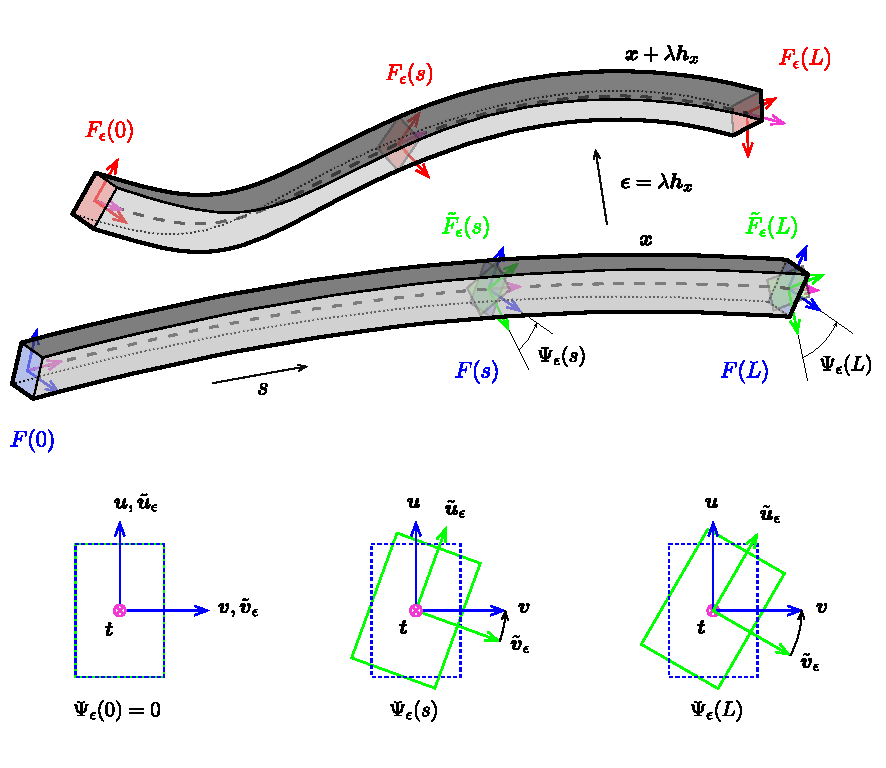
\includegraphics[width=\linewidth]{writhe.pdf}
\caption{Repères de Frenet attachés à  $\gamma$.}
\label{fig:1_1}
\end{figure}

\subsubsection{Calculation of $\Psi_\epsilon$}

\begin{figure}[p]
\centering
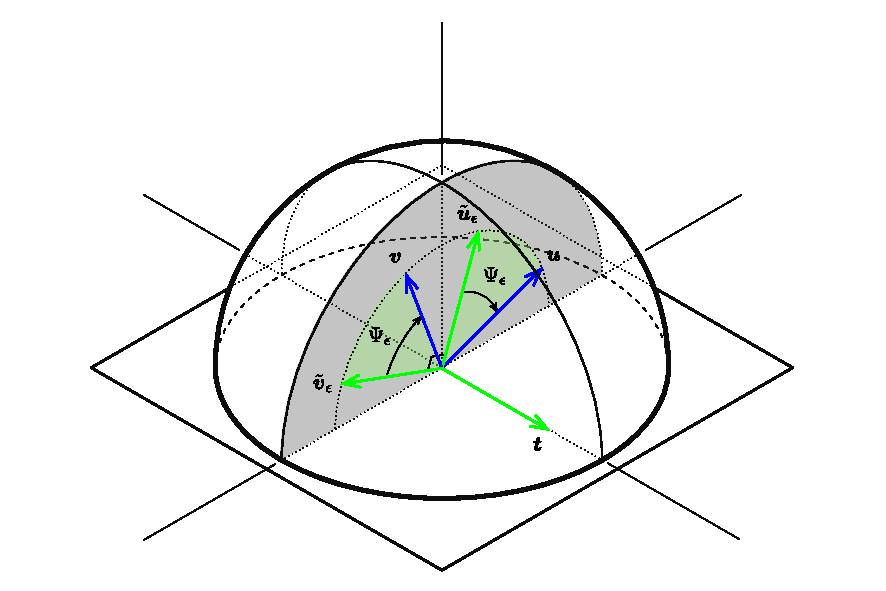
\includegraphics[width=\textwidth]{rotation_A.pdf}
\caption{$F$ is obtained by rotating $\tilde{F}_\epsilon$ around $\vect{t}$ of an angle $\Psi_\epsilon$.}
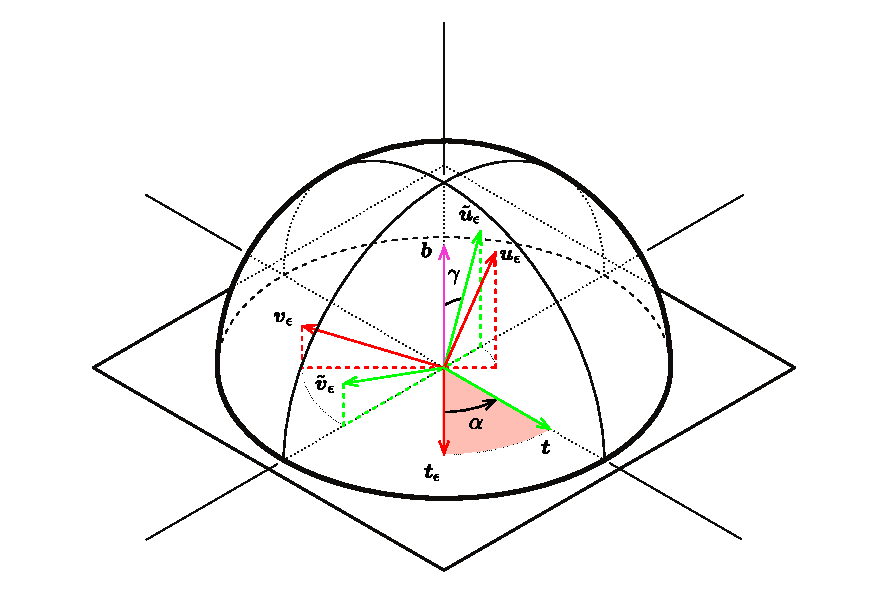
\includegraphics[width=\textwidth]{rotation_B.pdf}
\caption{$\tilde{F}_\epsilon$ is obtained by parallel tranpsporting $F_\epsilon$ from $\vect{t}_\epsilon$ to $\vect{t}$. This operation could be seen as a rotation around $\vect{t}_\epsilon \times \vect{t}$ of an angle $\alpha_\epsilon$.}
\label{A}
\end{figure}

This variation is closely related to the writhe of closed curves. As explained in \cite{Fuller1978} when parallel transporting an adapted frame around a closed curve it might not realigned with itself after one complete loop. This \guil{lack of alignement} is directly measured by the change of writhe which can be computed with Fuller's Formula \cite{Fuller1978}.

Note that the derivative of $\theta$ with respect to $\vect{x}$ can be evaluated by the change of writhe in the curve as suggested in \cite{deVries2005}. This approach is completly equivalent.

One can also see this lack of alignement in terms of rotation. Parallel transport being a propagation of frame from $s = 0$, the cumulated rotation of Bishop frame from the deformed configuration around the initial configuration at arc-length $s$ is the cumulated angle of rotation of $\vect{u}[\vect{x} + \lambda\vect{h}_x]$ around $\vect{d}_3[\vect{x}]$. Recalling the rotation rate of $\vect{u}[\vect{x} + \lambda\vect{h}_x]$ is $\kappa\vect{b}[\vect{x} + \lambda\vect{h}_x]$ by definition of zero-twisting frame, one can write :
\begin{equation}
	\Psi_\epsilon[\vect{x}](s) =
	-\int_0^s \kappa\vect{b}[\vect{x} + \lambda\vect{h}_x] \cdot \vect{d}_3[\vect{x}] \,dt
\end{equation}
The calculation of $\kappa\vect{b}[\vect{x} + \lambda\vect{h}_x]$ is straight forward from the curvature binormal definition :
\begin{equation}
	\begin{aligned}
	\kappa\vect{b}[\vect{x} + \lambda\vect{h}_x]
	&= (\vect{x} + \lambda\vect{h}_x)' \times (\vect{x} + \lambda\vect{h}_x)'' \\
	&= \kappa\vect{b}[\vect{x}] + \lambda(\vect{x}'\times\vect{h}''_x + \vect{h}'_x\times\vect{x}'') + \lambda^2(\vect{h}'_x \times \vect{h}''_x) \\
	&= \kappa\vect{b}[\vect{x}] + \lambda(\vect{x}'\times\vect{h}''_x + \vect{h}'_x\times\vect{x}'') + o(\lambda)
	\end{aligned}
\end{equation}
Thus, reminding that $\vect{d}_3[\vect{x}] = \vect{x}'$ and $\kappa\vect{b}[\vect{x}]\cdot\vect{d}_3[\vect{x}] = 0$, and using the invariance of circular product by cyclic permutation, one can express :
\begin{equation}
	\begin{aligned}
		\Psi_\epsilon[\vect{x}](s)
		&= -\int_0^s \kappa\vect{b}[\vect{x} + \lambda\vect{h}_x] \cdot \vect{d}_3[\vect{x}] \,dt\\
		&= - \lambda \int_0^s (\vect{x}'\times\vect{h}''_x + \vect{h}'_x\times\vect{x}'') \cdot \vect{x}' \,dt + o(\lambda)\\
		&= - \lambda \int_0^s \kappa\vect{b}[\vect{x}]\cdot\vect{h}'_x \,dt + o(\lambda)\\
	\end{aligned}
\end{equation}
By integration by parts, dropping the implicit reference to $\vect{x}$ in the notation, and denoting by $\delta_s$ and $H_s$ the Dirac function and the Heaviside step function centered at $s$, $\Psi_\epsilon(s)$ could be rewritten as :
\begin{equation}
	\begin{aligned}
		\Psi_\epsilon(s)
		&= - \lambda \int_0^s \kappa\vect{b}\cdot\vect{h}'_x \,dt + o(\lambda)\\
		&=  - \lambda \left(\big[\kappa\vect{b} \cdot  \vect{h}_x \big]_0^s - \int_0^s \kappa\vect{b}' \cdot  \vect{h}_x \,dt\right) + o(\lambda)\\
		&= - \lambda \left(\int_0^s \left(\left(\delta_s-\delta_0\right)\kappa\vect{b} - \kappa\vect{b}'\right)\cdot  \vect{h}_x \,dt\right) + o(\lambda)\\
		&= - \lambda \left(\int_0^L \left(\left(\delta_s-\delta_0\right)\kappa\vect{b} - (1-H_s)\kappa\vect{b}'\right)\cdot  \vect{h}_x \,dt\right) + o(\lambda)
	\end{aligned}
\end{equation}
Note that, as expected, $\Psi_\epsilon(s)$ is in first order of $\lambda$ and thus gets negligible when $\lambda$ tends to zero, that is to say when the perturbation of $\vect{x}$ is infinitesimal :
\begin{equation}
	\lim_{\lambda \to 0} \Psi_\epsilon(s) = 0
\end{equation}

$H_s : t \mapsto \left\{\begin{array}{c}0  , \quad t<s \\1  , \quad t\geqslant s \end{array}\right.$ est la fonction de Heaviside.

$\delta_s : t \mapsto \delta(t-s)$ est la distribution de dirac centrée en $s$.

\subsubsection{Calculation of $\alpha_\epsilon$}

Recall that $\tilde{F}_\epsilon$ is obtained by parallel tranpsporting $F_\epsilon$ from $\vect{t}_\epsilon$ to $\vect{t}$.
$\tilde{F}_\epsilon$ results from the rotation of $F_\epsilon$ around $\vect{b} = \vect{t}_\epsilon \times \vect{t}$ by an angle $\alpha_\epsilon$.

Recall from \eqref{eq:3_6} that because the rod is supposed to be unstretchable, $\vect{t}_\epsilon$ stays collinear to $\vect{t}$ for an infinitesimal perturbation of the centerline :
\begin{equation}
		\|\vect{t}\| = \|\vect{t}_\epsilon\| = 1
		\Rightarrow  (\vect{x}+\vect{\epsilon})' \cdot (\vect{x}+\vect{\epsilon})' = 1
		\Leftrightarrow  \vect{x}'\cdot\vect{\epsilon}' = - \tfrac{\lambda^2}{2}\|\vect{h}_x'\|^2
\end{equation}
Which leeds to :
\begin{equation}
		\cos \alpha_\epsilon(s) = \vect{t} \cdot \vect{t}_\epsilon = \vect{x}' \cdot (\vect{x}+\vect{\epsilon})'
		= 1 + \vect{x}' \cdot \vect{\epsilon}'
		= 1 - \tfrac{\lambda^2}{2}\|\vect{h}_x'\|^2
\end{equation}

Thus, at second order in $\lambda$ :
\begin{subequations}
	\begin{gather}
		\cos \alpha_\epsilon = 1 - \tfrac{\lambda^2}{2}\|\vect{h}_x'\|^2
		\\
		\sin \alpha_\epsilon = \sqrt{1-\cos^2 \alpha_\epsilon} = \lambda\|\vect{h}_x'\| + o(\lambda^2)
		\\
		\sin^2 {\alpha_\epsilon}{/2} = \tfrac{\lambda^2}{4}\|\vect{h}_x'\|^2
	\end{gather}
\end{subequations}

Finally, it's possible to conclude that $\alpha_\epsilon(s)$ is in first order of $\lambda$ and thus gets negligible when $\lambda$ tends to zero :
\begin{equation}
	\lim_{\lambda \to 0} \alpha_\epsilon(s) = 0
\end{equation}

%\begin{figure}[t]
%\centering
%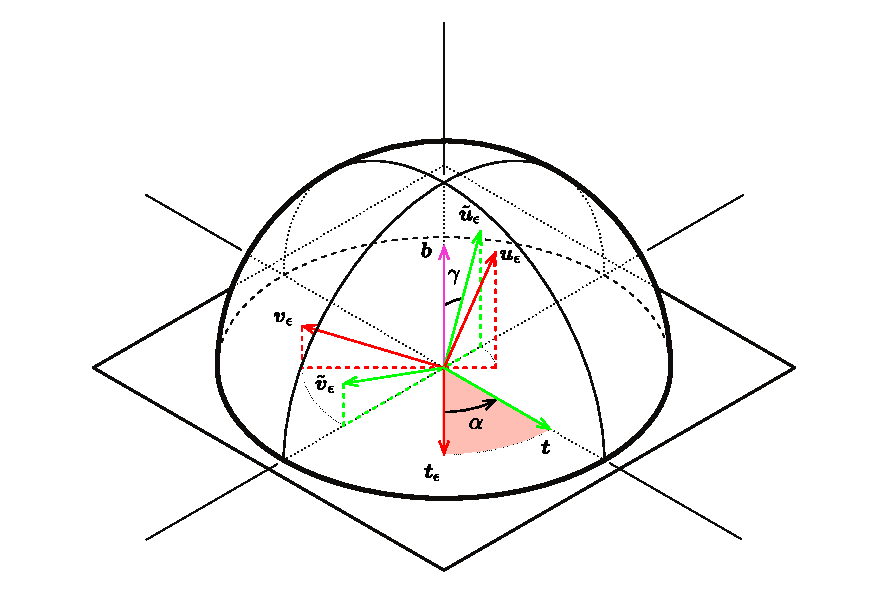
\includegraphics[width=\linewidth]{rotation_B.pdf}
%\caption{$\tilde{F}_\epsilon$ is obtained by parallel tranpsporting $F_\epsilon$ from $\vect{t}_\epsilon$ to $\vect{t}$. This operation could be seen as a rotation around $\vect{t}_\epsilon \times \vect{t}$ of an angle $\alpha$.}
%\label{fig:1_1}
%\end{figure}

\subsubsection{Aligning $\tilde{F}_\epsilon$ towards $F_\epsilon$}
Recall that aligning $\tilde{F}_\epsilon$ over $F$ is nothing but a rotation around $\vect{t}$ by an angle $\Psi_\epsilon$. This leads to :
\begin{subequations}
%	\left\{
	\begin{gather}
		\vect{\tilde{u}}_\epsilon = \cos{\Psi_\epsilon}\;\vect{u} + \sin{\Psi_\epsilon}\;\vect{v}\\
		\vect{\tilde{v}}_\epsilon = -\sin{\Psi_\epsilon}\;\vect{u} + \cos{\Psi_\epsilon}\;\vect{v}
	\end{gather}
%	\right.
\end{subequations}

\subsubsection{Aligning $F_\epsilon$ towards $\vect{t}$}

Recall that $\tilde{F}_\epsilon$ is obtained by parallel tranpsporting $F_\epsilon$ from $\vect{t}_\epsilon$ to $\vect{t}$. This operation could be seen as a rotation around $\vect{t}_\epsilon \times \vect{t}$ of an angle $\alpha_\epsilon$. Where :
\begin{equation}
	\vect{b} = \vect{t}_\epsilon \times \vect{t}
	 = \cos{\gamma}\;\vect{\tilde{u}}_\epsilon + \sin{\gamma}\;\vect{\tilde{v}}_\epsilon
	 = \cos{\gamma}\;\vect{u}_\epsilon + \sin{\gamma}\;\vect{v}_\epsilon
\end{equation}
Expressing $F_\epsilon$ on the basis $\tilde{F}_\epsilon$ gives for $\vect{u}_\epsilon$ and $\vect{v}_\epsilon$ :
\begin{subequations}
\begin{gather}
		\vect{u}_\epsilon = \sin{\gamma}\;\vect{b} + \cos{\gamma}\;\big(\sin{\alpha_\epsilon}\;\vect{\tilde{t}}
	+ \cos{\alpha_\epsilon}\;(\cos{\gamma}\;\vect{\tilde{u}_\epsilon}
	- \sin{\gamma}\;\vect{\tilde{v}_\epsilon})\big) 
		\\
		\vect{v}_\epsilon = \cos{\gamma}\;\vect{b} + \sin{\gamma}\;\big(-\sin{\alpha_\epsilon}\;\vect{\tilde{t}}
	+ \cos{\alpha_\epsilon}\;(\sin{\gamma}\;\vect{\tilde{u}_\epsilon}
	- \cos{\gamma}\;\vect{\tilde{v}_\epsilon})\big) 
\end{gather}
\end{subequations}
Which can be rearranged in :
\begin{subequations}
\begin{gather}
		\vect{u}_\epsilon = \cos{\gamma}\sin{\alpha_\epsilon}\;\vect{t}
	+ (\cos{\alpha_\epsilon}\cos^2{\gamma}+ \cos^2{\gamma})\vect{\tilde{u}_\epsilon}
	+ \sin{\gamma}\cos{\gamma}\;(1-\cos{\alpha_\epsilon})\vect{\tilde{v}_\epsilon}
		\\
		\vect{v}_\epsilon = -\sin{\gamma}\sin{\alpha_\epsilon}\;\vect{t}
	+ \cos{\gamma}\sin{\gamma}\;(1-\cos{\alpha_\epsilon})\vect{\tilde{u}_\epsilon}
	+ (\cos^2{\gamma} + \cos{\alpha_\epsilon}\sin^2{\gamma})\vect{\tilde{v}_\epsilon}
\end{gather}
\end{subequations}

\subsubsection{Variation of Bishop frame with respect to $\vect{x}$}
Finally, one can express $F_\epsilon$ on the basis $F$ as the composition of two rotations :
\begin{subequations}
	\begin{gather}
	\vect{u}_\epsilon =
	\begin{bmatrix}
		1 & 0 & 0 \\
		0 & \cos{\Psi_\epsilon} & -\sin{\Psi_\epsilon} \\
		0 & \sin{\Psi_\epsilon} & \cos{\Psi_\epsilon}
	\end{bmatrix}
	\begin{bmatrix}
		\cos{\gamma}\sin{\alpha_\epsilon} \\
		1-2\cos^2{\gamma}\sin^2{\alpha_\epsilon/2} \\
		2\sin{\gamma}\cos{\gamma}\sin^2{\alpha_\epsilon/2}
	\end{bmatrix}
	=
	\begin{bmatrix}
		\alpha_\epsilon\cos{\gamma}\\
		1 \\
		\Psi_\epsilon
	\end{bmatrix}
	+ o(\lambda)
	\\
	\vect{v}_\epsilon =
	\begin{bmatrix}
		1 & 0 & 0 \\
		0 & \cos{\Psi_\epsilon} & -\sin{\Psi_\epsilon} \\
		0 & \sin{\Psi_\epsilon} & \cos{\Psi_\epsilon}
	\end{bmatrix}
	\begin{bmatrix}
		-\sin{\gamma}\sin{\alpha_\epsilon} \\
		2\sin{\gamma}\cos{\gamma}\sin^2{\alpha_\epsilon/2} \\
		1-2\sin{\gamma}^2\sin^2{\alpha_\epsilon/2}
	\end{bmatrix}
	=
	\begin{bmatrix}
		-\alpha_\epsilon\sin{\gamma}\\
		-\Psi_\epsilon \\
		1
	\end{bmatrix}
	+ o(\lambda)
	\end{gather}
\end{subequations}

%\begin{equation}
%
%\end{equation}
Here, the expressions have been developed in first order of $\lambda$ as far as $\alpha_\epsilon$ and $\Psi_\epsilon$ it's been proofed in eq [] that those quantities tends two zero when the perturbation of the centerline is infinitesimal.

Finally, one can express the variation of material directors with respect to an infinitesimal variation of rod's centerline :
\begin{subequations}
\begin{gather}
		\vect{u}_\epsilon = \alpha_\epsilon\cos{\gamma}\;\vect{t} + \vect{u} + \Psi_\epsilon\vect{v} + o(\lambda)
		\\
		\vect{v}_\epsilon = -\alpha_\epsilon\sin{\gamma}\;\vect{t} + \vect{v} - \Psi_\epsilon\vect{u} + o(\lambda)
\end{gather}
\end{subequations}

\subsubsection{Variation of material frame with respect to $\vect{x}$}
Recalling the expression of the material frame expressed in the reference Bishop frame, it's now easy to deduce the variation of material frame with respect to a variation of the rod's centerline :
\begin{subequations}
		\begin{gather}
			\vect{d}_1[\vect{x}+\lambda \vect{h}_x] =
			\cos{\theta} \; \vect{u}_\epsilon + \sin{\theta} \; \vect{v}_\epsilon\\
			\vect{d}_2[\vect{x}+\lambda \vect{h}_x] =
			-\sin{\theta} \; \vect{u}_\epsilon + \cos{\theta} \; \vect{v}_\epsilon
		\end{gather}
\end{subequations}
Which leads according to the previous equation to :
\begin{subequations}
	\begin{gather}
		\vect{d}_1[\vect{x}+\lambda \vect{h}_x] = \vect{d}_1[\vect{x}] + \Psi_\epsilon\vect{d}_2[\vect{x}] + \alpha_\epsilon\cos{(\theta-\gamma)}\;\vect{t}[\vect{x}] + o(\lambda) \\
		\vect{d}_2[\vect{x}+\lambda \vect{h}_x] = \vect{d}_2[\vect{x}] - \Psi_\epsilon\vect{d}_1[\vect{x}] - \alpha_\epsilon\sin{(\theta+\gamma)}\;\vect{t}[\vect{x}] + o(\lambda)
		\end{gather}
\end{subequations}

\subsection{Derivative of the material curvatures vector with respect to $\vect{x}$}

It's know straightforward from the previous section to express the variation of the material curvatures with respect to a variation $\vect{\epsilon} =\lambda \vect{h}_x$ of $\vect{x}$ while $\theta$ remains unchanged.
\begin{subequations}
	\begin{gather}
		(\vect{x}+\lambda \vect{h}_x)'' \cdot \vect{d}_1[\vect{x}+\lambda \vect{h}_x] =
			(\vect{x}''+\lambda \vect{h}_x'')\cdot\big(\vect{d}_1 + \Psi_\epsilon\vect{d}_2
			+ \alpha_\epsilon\cos{(\theta-\gamma)}\;\vect{t} + o(\lambda)\big) \\
		(\vect{x}+\lambda \vect{h}_x)'' \cdot \vect{d}_2[\vect{x}+\lambda \vect{h}_x] =
			(\vect{x}''+\lambda \vect{h}_x'')\cdot\big(\vect{d}_2 - \Psi_\epsilon\vect{d}_1
			- \alpha_\epsilon\sin{(\theta+\gamma)}\;\vect{t} + o(\lambda)\big)
		\end{gather}
\end{subequations}
Thus, recalling that $\vect{x}''\cdot\vect{d}_3 = 0$ and that $\alpha_\epsilon$ and $\Psi_\epsilon$ are first order quantities in $\lambda$ :
\begin{subequations}
	\begin{gather}
		(\vect{x}+\lambda \vect{h}_x)'' \cdot \vect{d}_1[\vect{x}+\lambda \vect{h}_x] = 					\vect{x}''\cdot\vect{d}_1 + \Psi_\epsilon\vect{x}''\cdot\vect{d}_2 + \lambda \vect{h}_x''\cdot\vect{d}_1 + o(\lambda)\\
		(\vect{x}+\lambda \vect{h}_x)'' \cdot \vect{d}_2[\vect{x}+\lambda \vect{h}_x] =
				\vect{x}''\cdot\vect{d}_2 - \Psi_\epsilon\vect{x}''\cdot\vect{d}_1 +  \lambda \vect{h}_x''\cdot\vect{d}_2 + o(\lambda)
	\end{gather}
\end{subequations}
Which finally leads to :
\begin{equation}
		\vect{\omega}[\vect{x}+\lambda \vect{h}_x]  =
		\vect{\omega}[\vect{x}] - \Psi_\epsilon\mat{J}\vect{\omega}[\vect{x}]+\lambda
		\begin{bmatrix}
			-\vect{h}_x''\cdot\vect{d}_2\\
			\vect{h}_x''\cdot\vect{d}_1\\
		\end{bmatrix} + o(\lambda)
\end{equation}
Reminding the expression of $\Psi_\epsilon$ computed in paragraphe[], one can express the derivative of the material curvatures vector with respect to $\vect{x}$ :
\begin{equation}
			\pdiffof{x}{\vect{\omega}}{s}{\vect{h}_x}
	= 	\left(\int_0^L \left(\left(\delta_s-\delta_0\right)\kappa\vect{b} - (1-H_s)\kappa\vect{b}'\right)\cdot  \vect{h}_x \,dt\right)\mat{J}\vect{\omega}+
		\begin{bmatrix}
			-{\vect{d}_2}^T\\
			{\vect{d}_1}^T\\
		\end{bmatrix}\cdot \vect{h}_x''
\end{equation}


\subsection{Computation of the forces acting on the centerline}

The forces acting on the centerline are given by the functional derivative of the potential elastic energy with respect to $x$ which can be decomposed according to the chaine rule :
\begin{equation}
	\begin{aligned}
	\scalar{-f(s)}{\vect{h}_x} = \pdiffof{x}{\mathcal{E}_p}{s}{\vect{h}_x}
	&= \pdiffof{x}{\mathcal{E}_b}{s}{\vect{h}_x} + \pdiffof{x}{\mathcal{E}_t}{s}{\vect{h}_x} \\
	&= \pdiffof{x}{\mathcal{E}_b[\vect{\omega}[\vect{x}]]}{s}{\vect{h}_x} + \pdiffof{x}{\mathcal{E}_t[\vect{x}]}{s}{\vect{h}_x} \\
	\end{aligned}
\end{equation}

\subsubsection{Derivative of the torsion energy with respect to $x$}

Recall that the torsion energy only depends on $\theta$ which is independent of $x$. Thus, $\mathcal{E}_t$ is independent of $x$ :
\begin{equation}
	\pdiffof{x}{\mathcal{E}_t[\vect{x}]}{s}{\vect{h}_x}
		= \frac{d}{d\lambda} \mathcal{E}_t[\vect{x} + \lambda \vect{h}_x]\Bigr|_{\lambda = 0} = 0
\end{equation}

\subsubsection{Derivative of the bending energy with respect to $x$}

The derivative of $\mathcal{E}_b$ is obtained with the chaine rule :
\begin{equation}
	\pdiffof{\omega}{\mathcal{E}_b[\vect{\omega}]}{s}{\vect{h}_\omega}
		= \frac{d}{d\lambda} \mathcal{E}_b[\vect{\omega} + \lambda \vect{h}_\omega]\Bigr|_{\lambda = 0}
		= \int_{0}^{L} (\vect{\omega} - \overbar{\vect{\omega}})^T \mat{B} \cdot \vect{h}_\omega \;dt
\end{equation}
Finally, reminding eq 4.14 :
\begin{equation}
	\pdiffof{x}{\mathcal{E}_b[\vect{\omega}[\vect{x}]]}{s}{\vect{h}_x}
	= \pdiffof{\omega}{\mathcal{E}_b[\vect{\omega}]}{s}{(\pdiffof{x}{\vect{\omega}[\vect{x}]}{s}{\vect{h}_x})}
	= \mathcal{A} +\mathcal{B}+\mathcal{C}
\end{equation}
Where :
\begin{subequations}
	\begin{gather}
	\mathcal{A} = \int_{0}^{L} (\vect{\omega} - \overbar{\vect{\omega}})^T \mat{B}
	\begin{bmatrix}
		-{\vect{d}_2}^T\\
		{\vect{d}_1}^T\\
	\end{bmatrix}\cdot \vect{h}_x'' \;dt \\
	\mathcal{B} =
	\int_{t=0}^{L} (\vect{\omega} - \overbar{\vect{\omega}})^T \mat{B}\mat{J}\vect{\omega}
	\left(\int_{u=0}^L \left(\delta_t-\delta_0\right)\kappa\vect{b}\cdot  \vect{h}_x \;du\right)
	\;dt\\
	\mathcal{C} =
	\int_{t=0}^{L} -(\vect{\omega} - \overbar{\vect{\omega}})^T \mat{B}\mat{J}\vect{\omega}
	\left(\int_{u=0}^L \left(1-H_t\right)\kappa\vect{b}'\cdot  \vect{h}_x \;du\right)
	\;dt
	\end{gather}
\end{subequations}

Calculus of $\mathcal{A}$ :
\begin{equation}
	\mathcal{A}
	= \int_{0}^{L} (\vect{\omega} - \overbar{\vect{\omega}})^T \mat{B}
		\begin{bmatrix}
			-{\vect{d}_2}^T\\
			{\vect{d}_1}^T\\
		\end{bmatrix}\cdot \vect{h}_x'' \;dt \\
\end{equation}

Recalling the bending moment is given by : 
\begin{equation}
	\vect{M}  
	= (\kappa_1 - \overbar{\kappa_1})EI_1\vect{d}_1 + (\kappa_2 - \overbar{\kappa_2})EI_2\vect{d}_2
	= M_1\vect{d}_1 + M_2\vect{d}_2
\end{equation}
One can remark that :
\begin{equation}
	\left(\vect{\omega} - \overbar{\vect{\omega}}\right)^T \mat{B} 
		\begin{bmatrix}
			-{\vect{d}_2}^T\\
			{\vect{d}_1}^T\\
		\end{bmatrix}
	=  M_2{\vect{d}_1}^T - M_1{\vect{d}_2}^T
	= - ({\vect{d}_3} \times \vect{M})^T
\end{equation}

\note{
Rq : on mixe abusivement 2 formes d'écritures, matricielle et vectorielle, à cause du produit scalaire que l'on écrit tantôt sous sa forme vectorielle et parfois matricielle (à l'aide de la transposée).}

Thus,  $\mathcal{A}$ could be rewritten in it's vectoriel form :
\begin{equation}
	\begin{aligned}
	\mathcal{A}
	& = -\int_{0}^{L} ({\vect{d}_3} \times \vect{M}) \cdot \vect{h}_x'' \;dt \\
	& = -\left[\left({\vect{d}_3} \times \vect{M}\right) \cdot \vect{h}_x'\right]_0^L
		+ \int_{0}^{L} \left({\vect{d}_3} \times \vect{M}\right)'\cdot \vect{h}_x' \;dt \\
	& = -\left[\left({\vect{d}_3} \times \vect{M}\right) \cdot \vect{h}_x'\right]_0^L
		+ \int_{0}^{L} \left(
			\left({\vect{d}_3} \times \vect{M}'\right) \cdot \vect{h}_x'
			+ \left({\vect{h}'_x} \times \vect{d}_3'\right) \cdot \vect{M}
			 \right)\;dt \\
	\end{aligned}
\end{equation}
Recall that from \eqref{eq:3_6} that $\vect{h}'_x \cdot \vect{d}_3 = 0$  and from \eqref{eq:3_1} that $\vect{d}'_3 \cdot \vect{d}_3 = 0$. Hence, $\vect{h}'_x \times \vect{d}_3'$ is colinear to $\vect{d}_3$. Or by definition $\vect{M}$ is orthogonal to $\vect{d}_3$. Thus, $\left({\vect{h}'_x} \times \vect{d}_3'\right) \cdot \vect{M} = 0$.
Finally, after a second integration by parts :
\begin{equation}
	\begin{aligned}
	\mathcal{A}
	& = -\left[\left({\vect{d}_3} \times \vect{M}\right) \cdot \vect{h}_x'\right]_0^L
		+ \int_{0}^{L} \left(
			{\vect{d}_3} \times \vect{M}'\right) \cdot \vect{h}_x'
			 \;dt \\
	& = 	\left[
			({\vect{d}_3} \times \vect{M}') \cdot \vect{h}''_x\
			- ({\vect{d}_3} \times \vect{M}) \cdot \vect{h}_x'
		\right]_0^L
		- \int_{0}^{L} \left({\vect{d}_3} \times \vect{M}'\right)' \cdot \vect{h}_x \;dt \\
	\end{aligned}
\end{equation}

Calculus of $\mathcal{B}$ :
\begin{equation}
	\begin{aligned}
	\mathcal{B} &=
	\int_{t=0}^{L} (\vect{\omega} - \overbar{\vect{\omega}})^T \mat{B}\mat{J}\vect{\omega}
	\left(\int_{u=0}^L \left(\delta_t-\delta_0\right)\kappa\vect{b}\cdot  \vect{h}_x \,du\right)
	\;dt
	\\
	&=
	-\left(\kappa\vect{b}\cdot\vect{h}_x\right)(0) \int_{t=0}^{L} (\vect{\omega} - \overbar{\vect{\omega}})^T \mat{B}\mat{J}\vect{\omega}\;dt
	+
	\int_{t=0}^{L} (\vect{\omega} - \overbar{\vect{\omega}})^T \mat{B}\mat{J}\vect{\omega}
	\kappa\vect{b}\cdot\vect{h}_x
	\;dt
	\end{aligned}
\end{equation}

Calculus of $\mathcal{C}$ :
\begin{equation}
	\begin{aligned}
	\mathcal{C} &=
	\int_{t=0}^{L} -(\vect{\omega} - \overbar{\vect{\omega}})^T \mat{B}\mat{J}\vect{\omega}
	\left(\int_{u=0}^L \left(1-H_t\right)\kappa\vect{b}'\cdot  \vect{h}_x \;du\right)
	\;dt
	\\
	&=
	\int_{u=0}^{L}\int_{t=u}^{L}-\left((\vect{\omega} - \overbar{\vect{\omega}})^T \mat{B}\mat{J}\vect{\omega}\right)(t)
	\left(\kappa\vect{b}'\cdot \vect{h}_x\right)(u) \;dt\;du
	\\
	&=
	\int_{u=0}^{L}-\left(\int_{t=u}^{L}(\vect{\omega} - \overbar{\vect{\omega}})^T \mat{B}\mat{J}\vect{\omega}\;dt\right)
	\left(\kappa\vect{b}'\cdot \vect{h}_x\right)\;du
	\\
	\end{aligned}
\end{equation}
By several integration by parts, using Fubini's theorem once and supposing that the terms vanishes at $s=0$ and $s=L$ :
\begin{equation}
	\begin{aligned}
	\mathcal{B}+\mathcal{C} &=
	\int_{t=0}^{L} \left(
	(\vect{\omega} - \overbar{\vect{\omega}})^T \mat{B}\mat{J}\vect{\omega}
	\kappa\vect{b}
	-
	\left(\int_{u=t}^{L}(\vect{\omega} - \overbar{\vect{\omega}})^T \mat{B}\mat{J}\vect{\omega}\;du\right)
	\kappa\vect{b}'
	\right)\cdot \vect{h}_x \;dt\\
	&=
	\int_{t=0}^{L} \left(
	-\left(\int_{u=t}^{L}(\vect{\omega} - \overbar{\vect{\omega}})^T \mat{B}\mat{J}\vect{\omega}\;du\right)'
	\kappa\vect{b}
	-
	\left(\int_{u=t}^{L}(\vect{\omega} - \overbar{\vect{\omega}})^T \mat{B}\mat{J}\vect{\omega}\;du\right)
	\kappa\vect{b}'
	\right)\cdot \vect{h}_x \;dt\\
	&=
	\int_{t=0}^{L} \left(
	-\left(\int_{u=t}^{L}(\vect{\omega} - \overbar{\vect{\omega}})^T \mat{B}\mat{J}\vect{\omega}\;du\right)
	\kappa\vect{b}
	\right)'\cdot \vect{h}_x \;dt\\
	\end{aligned}
\end{equation}

Which can be rewritted using the quasi-static hypothesis :
\begin{equation}
	\begin{aligned}
	\mathcal{B}+\mathcal{C}
	&=
	\int_{t=0}^{L} \left(
	-\left(\int_{u=t}^{L}(\vect{\omega} - \overbar{\vect{\omega}})^T \mat{B}\mat{J}\vect{\omega}\;du\right)
	\kappa\vect{b}
	\right)'\cdot \vect{h}_x \;dt\\
	&=
	\int_{t=0}^{L} \left(
	-\left(
	\int_{u=t}^{L}\beta(\theta' -{\overbar{\theta'}})(\delta_L-\delta_0) - \left(\beta(\theta' -{\overbar{\theta'}})\right)'\;du
	\right)
	\kappa\vect{b}
	\right)'\cdot \vect{h}_x \;dt\\
	&=
	\int_{t=0}^{L} \left(
	-\left(
	\beta(\theta' -{\overbar{\theta'}})(L) - \left[\beta(\theta' -{\overbar{\theta'}})\right]_t^L
	\right)
	\kappa\vect{b}
	\right)'\cdot \vect{h}_x \;dt\\
		&=
	\int_{t=0}^{L} -\left(
	\beta(\theta' -{\overbar{\theta'}})
	\kappa\vect{b}
	\right)'\cdot \vect{h}_x \;dt\\
	\end{aligned}
\end{equation}

Finally :
\begin{equation}
		\pdiffof{x}{\mathcal{E}_b[\vect{\omega}[\vect{x}]]}{s}{\vect{h}_x}
		=
		\int_{0}^{L} \left(
		- \left({\vect{d}_3} \times \vect{M}'\right)' 
		- \left(\beta(\theta' -{\overbar{\theta'}}) \kappa\vect{b}\right)'
		\right)\cdot \vect{h}_x \;dt\\
\end{equation}

\subsubsection{Internal forces}

Thus, the internal forces are related to the variation of internal elastic energy as :
\begin{equation}
	\begin{aligned}
	\scalar{-\vect{f}(s)}{\vect{h}_x} &= \pdiffof{x}{\mathcal{E}_p}{s}{\vect{h}_x}
		=
		- \int_{0}^{L} \left(
		\left({\vect{d}_3} \times \vect{M}'\right)' 
		+ \left(\beta(\theta' -{\overbar{\theta'}}) \kappa\vect{b}\right)'
		\right)\cdot \vect{h}_x \;dt\\
	\end{aligned}
\end{equation}
Finally, we can conclude on the expression of the internal forces :
\begin{equation}
	\vect{f}(s) = \left({\vect{d}_3} \times \vect{M}'\right)' 
		+ \left(\beta(\theta' -{\overbar{\theta'}}) \kappa\vect{b}\right)'
\end{equation}
The shear force acting on the right side of a section is nothing but $\vect{T} = \int \vect{f}$ :
\begin{equation}
	\vect{T}(s) = \vect{d}_3 \times \vect{M}'
		+ \beta(\theta' -{\overbar{\theta'}}) \kappa\vect{b}
\end{equation}

\note{
Remarquer ici que l'expression est purement locale.
Elle ne dépend pas du sens de parcours de la poutre, contrairement au raisonnement suivi.
Cette différence est notable avec la démarche de B. Audoly.
Faire le bilan des bénéfices de l'hypothèse quasi-statique :
- expressions rigoureusement vraies à  l'équilibre statique
- simplification ds le calcul des efforts
- rapidité dans le calcul avec des expressions plus simples
- il n'est pas forcément intéressant en terme d'algorithmie d'imposer l'hypothèse quasistatique au cours du calcul. Il faudrait faire un bench pour savoir.
}

\section{Conclusion}

On retrouve les équations de kirchhoff dynamique où l'on a négligé les forces inertielles de rotation d'un élément de poutre autour de $\vect{d}_1$ et $\vect{d}_2$ pour ne garder que la dynamique de rotation de la section autour de la fibre neutre $\vect{d}_3$. 

\subsubsection{Constitutive Equations}
\begin{subequations}
	\begin{gather}
	\tau = \theta' \\
	Q = GJ(\tau -{\overbar{\tau}}) \\
	M1 = (\kappa_1-{\overbar{\kappa_1}})EI_1 \\
	M1 = (\kappa_2-{\overbar{\kappa_2}})EI_2 \\
	\vect{M} = M_1\vect{d}_1 + M_2\vect{d}_2 \\
	\vect{Q} = Q\vect{d}_3	
	\end{gather}
\end{subequations}

Notes : 
\begin{subequations}
	\begin{gather}
	\vect{d}_3 \cdot (\vect{M} \times \vect{d}_3) = \kappa_1 M_1 + \kappa_2 M_1 \\
	\vect{d}_3 \cdot (\kappa\vect{b} \times \vect{M}) = \kappa_1 M_2 - \kappa_2 M_1 \\
	(\vect{\omega} - \overbar{\vect{\omega}})^T \mat{B} \mat{J}\vect{\omega} 
	 = - \kappa\vect{b} \cdot (\vect{d}_3 \times \mat{M})
	 = \kappa_1 \mat{M}_2 -  \kappa_2 \mat{M}_1
	\end{gather}
\end{subequations}

\subsubsection{Axial Force}
\begin{equation}
	\vect{N} = (ES \epsilon) \vect{d}_3
\end{equation}

\subsubsection{Shear Force}
\begin{equation}
	\vect{T}= \vect{d}_3 \times \vect{M}'
		  + Q\kappa\vect{b}
\end{equation}
\subsubsection{Rotational Moment}
\begin{equation}
	\vect{\Gamma}(s) = (Q' + \kappa_1 M_2 - \kappa_2 M_1)\vect{d}_3
	= Q' \vect{d}_3 + \kappa\vect{b} \times \vect{M}
\end{equation}
\subsubsection{Quasistatic hypothesis}
\begin{equation}
	Q' + \kappa_1 M_2 - \kappa_2 M_1 \simeq 0
\end{equation}
\subsubsection{Inextensibility hypothesis}
\begin{subequations}
	\begin{gather}
	\|\vect{x}'\| = \|(\vect{x} + \vect{\epsilon})'\| = 1 \\
	\|\vect{e}_i\| = \|\overbar{\vect{e}_i}\|
	\end{gather}
\end{subequations}

% #######################################################
\section{Numerical Model}
% #######################################################

En fait il faut faire quelques hypothèses sur la nature des efforts pour pourvoir les interpoler convenablement le long de la courbe. On va faire qqch qui ressemble à la super-clothoide de Bertails, et qui semble une hypothèse naturelle pour une poutre continue sur plusieurs appuis soumise à des forces et moments ponctuels :
\begin{itemize}
\item le moment est continu et linéaire par morceaux. Il est évalué ponctuellement aux noeuds et interpolé linéairement entre les noeuds.
\item la courbure est donc continue par morceaux et linéaire par morceaux. Elle est obtenue à partir du moment et de $\vect{B}$
\item N et Q sont constants par morceaux
\end{itemize}
\begin{subequations}
	\begin{gather}
		\vect{N}(s) = \vect{N}_{i}  \quad , \quad s \in ]0,|\vect{e}_i|[ \\
		\vect{M}(s) = \vect{M}_{i} + s \vect{M}'_{i} \quad s \in [0,|\vect{e}_i|]
		\quad , \quad \vect{M}'_{i}= \frac{\vect{M}_{i+1} - \vect{M}_{i}}{|\vect{e}_i|} \\
		\vect{Q}(s) = \vect{Q}_{i}  \quad , \quad s \in ]0,|\vect{e}_i|[ 
	\end{gather}
\end{subequations}

Faire un tableau vertex / edge quantities :
\begin{itemize}
\item les propriétés mécaniques sont définies aux noeuds
\item les repères matériels sont définis aux noeuds
\item les courbures sont définies aux noeuds
\item les moments sont définis aux noeuds et sont interpolés linéairement entre les noeuds
\item l'effort normal et le moment de torsion sont supposés uniformes sur les segments (ils sont donc définis aux segments)
\item $\alpha$ et $\beta$ sont des propriétés équivalentess définies sur les segments (égales à celles de noeuds s'il n'y a pas de saut de propriété).
\end{itemize}

\subsection{Force}

\subsubsection{Axial Force}

Axial Force exercée par la poutre sur le point courant $\vect{x}_i$ :
\begin{equation}
	\begin{aligned}
	\vect{F}_i^{\parallel}
	&= \left[\vect{N}\right]_{i-1/2}^{i+1/2}
	= \vect{N}_{i+1} - \vect{N}_{i}
	\end{aligned}
\end{equation}

Axial Force exercée par la poutre sur le premier point $\vect{x}_0$ :
\begin{equation}
	\begin{aligned}
	\vect{F}_i^{\parallel}
	&= \left[\vect{N}\right]_{0}
	= \vect{N}_{0}
	\end{aligned}
\end{equation}

Axial Force exercée par la poutre sur le dernier point $\vect{x}_n$ :
\begin{equation}
	\begin{aligned}
	\vect{F}_i^{\parallel}
	&= -\left[\vect{N}\right]_{0}
	= -\vect{N}_{n}
	\end{aligned}
\end{equation}



\subsubsection{Shear Force}

Shear Force exercée par la poutre sur le point courant $\vect{x}_i$ :
\begin{equation}
	\begin{aligned}
	\vect{F}_i^{\perp}
	&= \left[\vect{d}_3 \times \mat{M}' + Q\kappa\vect{b} \right]_{i-1/2}^{i+1/2} \\
	&= 	\frac{\vect{e}_i}{|\vect{e}_i|} \times \frac{\mat{M}_{i+1} - \mat{M}_{i}}{|\vect{e}_i|}
		- \frac{\vect{e}_{i-1}}{|\vect{e}_{i-1}|} \times \frac{\mat{M}_{i} - \mat{M}_{i-1}}{|\vect{e}_{i-1}|}
		+ Q_i\kappa\vect{b}^{-}_{i+1/2}
		- Q_{i-1}\kappa\vect{b}^{+}_{i-1/2}\\
	&= (\vect{F}^1_{i} + \vect{F}^2_{i} + \vect{H}^{-}_{i}) - (\vect{F}^1_{i-1} + \vect{F}^2_{i-1} +  \vect{H}^{+}_{i-1})
	\end{aligned}
\end{equation}

\note{Ici, on a un problème de définition de $\kappa\vect{b}$ en milieu de segment. En effet, bien que le moment soit continu, la courbure ne l'est pas nécessairement. Lorsqu'il y a un saut de $EI$ il y a nécessairement un saut de $\kappa\vect{b}$. On pourrait plutôt interpoler le moment à mi-travée et remonter à la courbure - soit à gauche, soit à droite - en fonction des propriétés géométriques locales :
\begin{subequations}
	\begin{gather}
	\vect{M}_{i+1/2} = \frac{\vect{M}_{i} + \vect{M}_{i+1}}{2} \\
	\kappa\vect{b}^{-}_{i+1/2} = \mat{B}_i^{-1}\vect{M}_{i+1/2} \\
	\kappa\vect{b}^{+}_{i+1/2} = \mat{B}_{i+1}^{-1}\vect{M}_{i+1/2}\\
	\vect{H}^-_{i} = Q_i\kappa\vect{b}^{-}_{i+1/2} = Q_i \mat{B}_i^{-1}\vect{M}_{i+1/2}\\
	\vect{H}^+_{i} = Q_i\kappa\vect{b}^{+}_{i+1/2} = Q_i \mat{B}_{i+1}^{-1}\vect{M}_{i+1/2}
	\end{gather}
\end{subequations}

L'autre approche consiste à ignorer la discontinuité et à simplement prendre la moyenne :
\begin{subequations}
	\begin{gather}
	\kappa\vect{b}_{i+1/2} = \kappa\vect{b}^{-}_{i+1/2} = \kappa\vect{b}^{+}_{i+1/2} 
	= \frac{\kappa\vect{b}_{i} + \kappa\vect{b}_{i+1}}{2} \\
	\vect{H}^-_{i} = Q_i\kappa\vect{b}^{-}_{i+1/2} \\
	\vect{H}^+_{i} = Q_i\kappa\vect{b}^{+}_{i+1/2} \\
	\vect{H}^-_{i} = \vect{H}^+_{i} = \frac{\kappa\vect{b}_{i} + \kappa\vect{b}_{i+1}}{2}
	\end{gather}
\end{subequations}
Cette idée reste intéressante et élégante. Elle n'a de sens que pour une poutre à propriétés variables (sinon on a la continuité de la courbure également).
}

Shear Force  exercée par la poutre sur le premier point $\vect{x}_0$ :
\begin{equation}
	\begin{aligned}
	\vect{F}_0^{\perp} 
	&= \left[\vect{d}_3 \times \mat{M}'+ Q\kappa\vect{b}\right]_{0} \\
	&= \frac{\vect{e}_0}{|\vect{e}_0|} \times \frac{\mat{M}_{1} - \mat{M}_{0}}{|\vect{e}_0|} 
	+ Q_0\frac{\kappa\vect{b}_{0}}{2} \\
	& = \vect{F}^1_{0} + \vect{F}^2_{0}  +  \vect{H}^-_{0}  \\
	\end{aligned}
\end{equation}

Shear Force  exercée par la poutre sur le dernier point $\vect{x}_n$ :
\begin{equation}
	\begin{aligned}
	\vect{F}_n^{\perp} 
	&= - \left[ \vect{d}_3 \times \mat{M}'+ Q\kappa\vect{b}\right]_{n} \\
	&= - \frac{\vect{e}_{n-1}}{|\vect{e}_{n-1}|} \times \frac{\mat{M}_{n} - \mat{M}_{n-1}}{|\vect{e}_{n-1}|} 
	- Q_n\frac{\kappa\vect{b}_{n}}{2} \\
	& = -(\vect{F}^1_{n} + \vect{F}^2_{n}  +  \vect{H}^+_{n}) \\
	\end{aligned}
\end{equation}


\subsubsection{Moment of Torsion}

\begin{equation}
	\begin{aligned}
	\Gamma_i 
		&= \int_{i-1/2}^{i-1/2} m(s)  
		= Q_{i} - Q_{i-1}
		+ \int_{i-1/2}^{i+1/2} \kappa_{1} M_{2} - \kappa_{2} M_{1}\\
		&= Q_{i} - Q_{i-1} + 
		+ \frac{\vect{e}_{i-1}}{|\vect{e}_{i-1}|} \cdot (\kappa\vect{b}_i \times \vect{M}^g_i )
		+ \frac{\vect{e}_i}{|\vect{e}_i|} \cdot (\kappa\vect{b}_i \times \vect{M}^d_i )
	\end{aligned}
\end{equation}




With
\begin{subequations}
	\begin{gather}
	[EI]_i \\ 
	[GJ]_i \\
	\kappa\vect{b}_i = \frac{2 \vect{e}_{i-1} \times \vect{e}_{i}}{|\vect{e}_{i-1}| |\vect{e}_i| |\vect{e}_{i-1} + \vect{e}_{i}|} \\
	\tau_i		= \frac{\theta_{i+1} - \theta_i}{|\vect{e}_i|} \\
	\vect{N}_{i} = N_i\vect{d}_3  \quad where \quad N_i = \alpha_i \epsilon_i \quad \alpha_i = \frac{2 [ES]_i [ES]_{i+1}}{[ES]_i + [ES]_{i+1}}\\
	\vect{M}_{i} 	= [EI]_{1,i}(\kappa_{1,i} - \overbar{\kappa}_{1,i})\vect{d}_{1,i} + [EI]_{2,i}(\kappa_{2,i} - \overbar{\kappa}_{2,i})\vect{d}_{2,i} \\ 
	\vect{Q}_{i} = Q_i\vect{d}_3 \quad where \quad Q_i = \beta_i (\tau_i - \overbar{\tau_i}) \quad \beta_i = \frac{2 [GJ]_i [GJ]_{i+1}}{[GJ]_i + [GJ]_{i+1}}\\
	\vect{F}^{1}_{i} 	= - \frac{\vect{e}_i \times \mat{M}_i}{|\vect{e}_i|^2} \\
	\vect{F}^{2}_{i} 	= + \frac{\vect{e}_i \times \mat{M}_{i+1}}{|\vect{e}_i|^2} \\ 
	\vect{H}^-_{i} 	= Q_i\kappa\vect{b}^{-}_{i+1/2} \\
	\vect{H}^+_{i} 	= Q_i\kappa\vect{b}^{+}_{i+1/2} \\
	\end{gather}
\end{subequations}
\note{Ici il y a une ambiguité sur $M_i$ en fonction d'un éventuel changement de propriété méca $EI_1$ ou $EI_2$. En fait il faudrait préciser un moment à droite et un moment à gauche (ce qui correspond à la réalité). Le moment étant la courbure au noeud i pondérée par $2EI$ à droite ou à gauche

Toutes les discrétisations ne se valent pas ....

En fait, ça n'a pas vraiment de sens de définir $EI$ sur le segment. Le moment est continu. Donc il est uniquement défini par la donnée de la courbure en un noeud et du $EI$ associé à ce noeuds. Introduire un moment à gauche et un moment à droite est problématique.
Ce qui ce passe, pour une poutre isostatique simple qui change de $EI$ à mi-travée, c'est une discontinuité de courbure $y''$ alors que $y$ et $y'$ restent continues.
Donc il semble plus pertinent de définir $EI$ aux noeuds car notre modèle ne peut pas représenter des discontinuitées de courbure (ou alors il faut connecter des poutres entre-elles.

Pour la torsion, on peut s'en sortir également en définissant $\beta$ aux noeuds et en supposant $GJ$ constant entre $[i-1/2,i+1/2]$. Il y a donc (éventuellement) un saut de $\beta$ au milieu de chaque $\vect{e}_i$. 

On ne peut pas faire autrement que supposer la torsion uniforme entre 2 noeuds, c'est à dire une variation linéaire (par morceaux) de $\theta$. Et il y a donc une discontinuité potentielle aux noeuds.

On écrit la continuité du champs de torsion entre les noeuds $1$ et $2$ malgré le saut de $\beta$ :

A mi travée
\begin{equation}
	\begin{aligned}
	Q_{12} = Q_{mid} =  Q_{1}^+ = Q_{2}^-
	&= [GJ]_1\frac{\theta_{mid} - \theta_{1}}{|\vect{e}|/2}
	= [GJ]_2 \frac{\theta_{2} - \theta_{mid}}{|\vect{e}|/2}
	\end{aligned}
\end{equation}
D'où :
\begin{equation}
	\theta_{mid} = \frac{[GJ]_1}{[GJ]_1 + [GJ]_2}\theta_1 + \frac{[GJ]_2}{[GJ]_1 + [GJ]_2}\theta_2
\end{equation}
On en déduit :
\begin{equation}
	Q_{12} = Q_{mid} =  Q_{1}^+ = Q_{2}^-
	= \frac{2 [GJ]_1 [GJ]_2}{[GJ]_1 + [GJ]_2} (\frac{\theta_{2} - \theta_{1}}{|\vect{e}|})
\end{equation}
Donc il faut plutôt définit $Q_i$ la torsion uniforme sur le segment $\vect{e}_i$ comme :
\begin{equation}
	Q_i = \beta_i (\tau_i - \overbar{\tau_i}) \quad where \quad \beta_i = \frac{2 [GJ]_i [GJ]_{i+1}}{[GJ]_i + [GJ]_{i+1}}
\end{equation}

On retrouve bien le cas d'une poutre de propriété constante lorsque $[GJ]_i= [GJ]_{i+1} = GJ$ alors $\beta_i = GJ$.


De manière identique, on résonne pour l'effort axial entre deux noeuds 1 et 2 auxquels sont associés des raideurs axiales $[ES]_1$ et $[ES_2]$. On cherche la raideur équivalente connaissant uniquement l'allongement de l'ensemble du segment :
\begin{subequations}
	\begin{gather}
	N_1 = [ES]_1 \cdot \epsilon_1 \\
	N_2 = [ES]_2 \cdot \epsilon_2 \\
	N =  [ES]_2 \cdot \frac{\epsilon_1 + \epsilon_2}{2}
	\end{gather}
\end{subequations}

Avec : 
\begin{subequations}
	\begin{gather}
	\epsilon_1 = \frac{l_1 - l_0/2}{l_0/2} \\
	\epsilon_2 = \frac{l_2 - l_0/2}{l_0/2} \\
	\epsilon = \frac{l}{l_0} = \frac{\epsilon_1}{2} + \frac{\epsilon_2}{2}  \\
	\end{gather}
\end{subequations}

Thus,
 \begin{equation}
	N_i = N_1 = N_2 \quad \Rightarrow \quad  \alpha_i = \frac{2 [ES]_i [ES]_{i+1}}{[ES]_i + [ES]_{i+1}} 
\end{equation}


 }
 

\bibliographystyle{alpha}
\bibliography{../bibliography}
